% Тут используется класс, установленный на сервере Papeeria. На случай, если
% текст понадобится редактировать где-то в другом месте, рядом лежит файл matmex-diploma-custom.cls
% который в момент своего создания был идентичен классу, установленному на сервере.
% Для того, чтобы им воспользоваться, замените matmex-diploma на matmex-diploma-custom
% Если вы работаете исключительно в Papeeria то мы настоятельно рекомендуем пользоваться
% классом matmex-diploma, поскольку он будет автоматически обновляться по мере внесения корректив
%

% По умолчанию используется шрифт 14 размера. Если нужен 12-й шрифт, уберите опцию [14pt]
\newcommand\tab[1][1cm]{\hspace*{#1}}
\documentclass[14pt]{matmex-diploma}
%\documentclass[14pt]{matmex-diploma-custom}

\begin{document}
% Год, город, название университета и факультета предопределены,
% но можно и поменять.
% Если англоязычная титульная страница не нужна, то ее можно просто удалить.
\filltitle{ru}{
    chair              = {Математическое обеспечение и администрирование информационных систем},
    title              = {Реализация возможности сжатия строки в КС-грамматику в YaccConstructor},
    % Здесь указывается тип работы. Возможные значения:
    %   coursework - Курсовая работа
    %   diploma - Диплом специалиста
    %   master - Диплом магистра
    %   bachelor - Диплом бакалавра
    type               = {coursework},
    position           = {студента},
    group              = 243,
    author             = {Зиновьева Анна Геннадьевна},
    supervisorPosition = {ст. преп, к. ф-м. н.},
    supervisor         = {Григорьев С.\,В.},
%   university         = {Санкт-Петербургский Государственный Университет},
%   faculty            = {Математико-механический факультет},
%   city               = {Санкт-Петербург},
%   year               = {2013}
}

\maketitle
\tableofcontents
% У введения нет номера главы
\section*{Введение}
    В информации очень часто можно наблюдать иерархические зависимости. Например, текст состоит из слов, фраз и предложений, которые могут повторяться, и намного выгоднее указать, что в нескольких местах у нас один и тот же фрагмент текста и описать его один раз, а не для каждого случая отдельно. Компьютерные программы состоят из модулей, функций, высказываний. Такие зависимости также можно увидеть в музыке. Также,  такой подход удобен в биоинформатике, например, при анализе и хранении ДНК и РНК, ведь они являются последовательностями символов из алфавита мощностью всего 4 элемента, а также имеют много общего у живых организмов, и чем ближе эти организмы биологически (из одного типа, семейства, рода и тем более, если родственники), тем больше одинаковых подпоследовательностей и, следовательно, зависимостей будет в их ДНК и РНК.
     
     YaccConstructor~\cite{YaccConstructorPage} --- исследовательский проект лаборатории языковых инструментов JetBrains, применяемого для задач лексического и синтаксического анализа. В нем уже реализованы интерфейсы для разбора грамматик в форматах .yrd, .g и .fsy . К существующей функциональности было решено добавить возможность построения грамматики из строки посредством нахождения в ней иерархических зависимостей. 

\section{Постановка задачи}
    Целью данной работы является реализация возможности сжатия текстовой строки в грамматику проекте YaccConstructor. 
    Были поставлены следующие задачи:
    \begin{itemize}
        \item реализовать алгоритм сжатия строки;
        \item реализовать возможность построения общей грамматики для нескольких строк;  
        \item реализовать конечное представление грамматики в формате \\YARD.IL~\cite{YARD};
        \item оформить фронтенд для данного алгоритма в рамках \\YaccConstructor;
        \item проверить эффективность данного решения.
    \end{itemize}
    
\section{Обзор}
	\subsection{Алгоритм Sequitur}
	Для решения данной задачи был предложен алгоритм Sequitur~\cite{sequitur} для сжатия последовательностей из дискретных символов. Данный алгоритм строит контекстно-свободную грамматику из последовательности символов, обрабатывая в ней все возможные повторы фрагментов. Контекстно-свободная грамматика --- грамматика с правилами вида: NonTerminal $\rightarrow$ sequence of (Terminal | NonTerminal). 
	
	Опишем суть алгоритма.
	Посимвольно сканируется последовательность терминалов, и строится список всех диграм (пар символов, стоящих рядом).
	Например, для строки “abcd” cписок диграм будет выглядеть так:
	
	[“ab”, “bc”, “cd”]

    У этого алгоритма есть два принципа:

    1. Уникальность --- никакая пара символов не встречается дважды. Каждый раз, когда какая-то пара символов появляется во второй раз, обе пары в последовательности заменяются на нетерминальный символ, список правил соответственно меняется, и алгоритм продолжает работу. 

    2. Полезность --- все правила используются не менее двух раз. Если же среди созданных нетерминалов встречается такой, что используется только один раз, то есть по сути является бесполезным, то он заменяется его определением.

    Рассмотрим работу алгоритма на строке “abcabc”.
    Будем сканировать строку и добавлять в список новые диграмы:

    S $\rightarrow$ a \tab digrams: [ ]
    
    S $\rightarrow$ ab \tab digrams: [“ab”] 
    
    S $\rightarrow$ abc	\tab digrams: [“ab”, “bc”]
    
    S $\rightarrow$ abca \tab digrams: [“ab”, “bc”, “ca”]
    
    S $\rightarrow$ abcab
    
    Вот тут мы получили новый диграм, который уже встречался раньше. Создаем новое правило A $\rightarrow$ ab, заменяем пары в последовательности и изменяем соответственно список диграм. То есть:
    
    S $\rightarrow$ AcA;  A $\rightarrow$ ab \tab digrams: [“Ac”, “cA”]
    
    S $\rightarrow$ AcAc
    
    Снова получили диграм, который уже встречался, создали правило B $\rightarrow$ Ac и заменили пары на нетерминал B. 
    
    S $\rightarrow$ BB;   B $\rightarrow$ Ac;   A $\rightarrow$ ab \tab digrams: [“BB”, ”Ac”, ”ab”]
    
    Но теперь правило A $\rightarrow$ ab используется только один раз, поэтому избавляемся от него.
    
    Таким образом, получаем:
    
    S $\rightarrow$ BB;   B $\rightarrow$ abc \tab digrams: [“BB”, ”ab”, ”bc”]
    
    Последний список правил и будет искомой грамматикой и результатом работы алгоритма.

	\subsection{YARD}
	    YARD --- язык спецификаций грамматик, являющийся частью \\YaccConstructor. Он позволяет использовать EBNF (Расширенную Форму Бэкуса-Наура), метаправила и условную генерацию. Также поддерживает грамматики с L и S атрибутами.
	    
	    Для описания конечного результата программы требуется два вида выражений: \begin{itemize}
	        \item выбор --- для реализации сжатия нескольких строк;
	        \item конкатенация --- для описания самих правил грамматики.
	        \end{itemize}  
	    
	    Поддерживая EBNF, YARD позволяет описывать контекстно-свободные грамматики, и, значит, позволяет представить результат алгоритма в нужной форме.

\section{Основная часть}

    \subsection{Реализация}
        Первый вопрос, который надо было решить, какой структурой можно представить грамматику. Нам необходимо выполнять следующие операции:
    \begin{enumerate}
        \item добавление символа в правило;
        \item замена двух терминальных символов на нетерминальный.
    \end{enumerate}
    Так как эти действия будут повторяться постоянно, нужна структура с эффективной поддержкой таких действий. Например, двусвязный список. В такой структуре оба действия будут выполняться за константное время.
    
    Во-вторых, когда мы находим диграм, который встречался уже до этого, мы подчиняем его правилу, после чего мы обязаны рассмотреть его соседей, если возможно подчинить их какому-либо правилу. То есть из состояния, когда мы рассматривали первый диграм, мы переходим в состояние рассмотрения соседних диграмов, которые тоже могут повлечь за собой просмотр уже их соседей. То есть образуется стек состояний, которые надо обработать. Этот принцип и был взят за основную функцию в реализации алгоритма, которая работает со стеком состояний.
    
    И третий вопрос, как реализовать возможность построения общей грамматики для нескольких последовательностей, склеенных через специальный символ (например, символ \&). Был найден такой выход.  Немного модифицируем алгоритм.
    При разборе стека состояний, каждый раз, когда нам встречается диграм, который содержит \&, мы не будем его обрабатывать: то есть не будем добавлять в список диграм, и, следовательно, смотреть, встречался ли такой диграм раньше (ведь его не может быть в списке). 
    Так как все диграмы, состоящие из обычных символов, стоящих перед и после специального символа \&, будут присутствовать в нашем списке, то, значит, они будут участвовать в образовании грамматики, и алгоритм будет работать корректно.
    
    Также, был оформлен интерфейс для алгоритма --- фронтенд к \\YaccConstructor. В нем реализована возможность сжать обычную строку, несколько строк, разделенных специальным символом, и массив строк. Представление YARD.IL, в виде которого возвращается грамматика, строится так:
    \begin{itemize}
        \item если символ терминальный, применяется конструктор PTok;
        \item если нетерминальный, то PRef;
        \item последовательность строится с помощью PSeq;
        \item а возможность сжатия нескольких строк реализуется через PAlt.
    \end{itemize}
    

    \subsection{Эксперимент}
    

    Для проверки эффективности данного решения была взята последовательность 16s РНК бактерий. Каждая последовательность состоит примерно из 1500 нуклеотидов, то есть последовательность символов из алфавита \{A; C; G; T\}
    \begin{figure}[h]
        \label{13} 
        \centering 
    	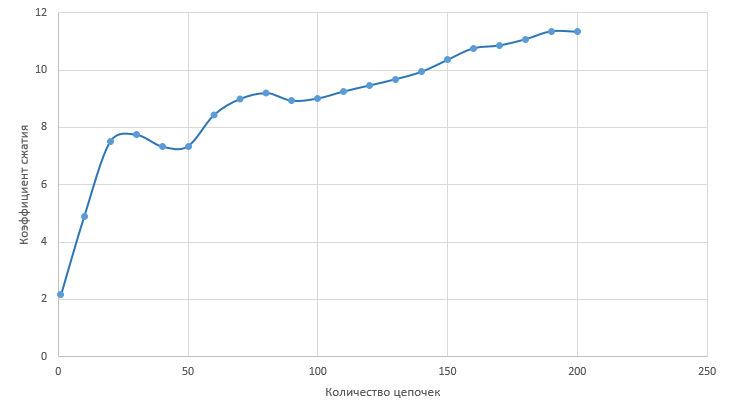
\includegraphics[width=1\textwidth]{pic1}
    	\caption{График зависимости сжатия входных данных}
    \end{figure}
    
    
    На графике показана зависимость коэффициента сжатия от количества сжимаемых последовательностей. Коэффициент сжатия вычисляется как отношение количества символов во всех последовательностях изначальных цепочек к количеству символов во всех правилах полученной грамматики. Как можно заметить, при сжатии небольшого количества строк, коэффициент получается маленьким, но потом быстро вырастает,  и дальше, при росте количества цепочек РНК, коэффициент тоже увеличивается, хотя и немного колеблется.
    \begin{figure}[h]
        \centering
    	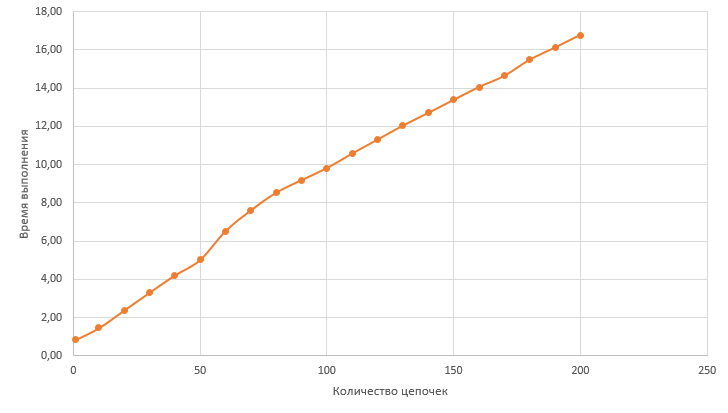
\includegraphics[width=1\textwidth]{pic2}
    	\caption{График зависимости времени выполнения программы}
    \end{figure}

    Это график зависимости времени выполнения программы от входных данных. На нем видно, что сложность реализованного алгоритма О(n). 
    
    Таким образом, можно назвать алгоритм достаточно эффективным.



% У заключения нет номера главы
\section{Заключение}
    В ходе данной работы было сделано следующее:
    \begin{itemize}
        \item реализован алгоритм Sequitur;
        \item реализована возможность построения общей грамматики для нескольких срок; 
        \item оформлен фронтенд к YaccConstructor для построения грамматики из строки в формате YARD.IL;
        \item проверена эффективность и производительность данного решения.
    \end{itemize}

    В дальнейшем планируется использовать данный проект для метагеномных сборок, а также компактного представления больших объемов данных.

\setmonofont[Mapping=tex-text]{CMU Typewriter Text}
\bibliographystyle{ugost2008ls}
\bibliography{diploma.bib}
\end{document}
